\section{Математическая модель динамики судна на нерегулярном волнении}

Для построения модели распределения сил и моментов, действующих на судно, морской объект рассматривается как твердое тело. Введем параметры, описывающие положение корабля в пространстве. Для этого необходимо выбрать локальную систему координат. За начало системы локальных координат примем центр тяжести корабля, а оси расположим так, чтобы ось $x$ была направлена вдоль корабля в направлении носовой части, ось $y$ – влево, ось $z$ – вверх, см. рис. ~\ref{boat_axis}.

\begin{figure}[ht]
\begin{center}
\includegraphics[width=110mm]{boat_axis}
\end{center}
\caption{Локальная система координат и углы вращения судна}
\label{boat_axis}
\end{figure}

Положение судна в пространстве однозначно определяется кортежем из вектора положения центра тяжести и вектора вращения: 
$P=(\mathbf{p},\mathbf{q})$, 
где  
$q=\alpha \mathbf{i}+\beta \mathbf{j}+\gamma \mathbf{k}$, 
где, в свою очередь $\alpha$, $\beta$, $\gamma$,  - углы крена, дифферента и курса, соответственно, а $\mathbf{i}$, $\mathbf{j}$, $\mathbf{k}$ – орты глобальной системы координат. Выпишем второй закон Ньютона:

\begin{equation}
	m \ddot{\mathbf{p}} = \mathbf{F}
	\label{ma=F}
\end{equation}

\begin{equation}
	\mathbf{J}  \ddot{\mathbf{p}} = \mathbf{M}
	\label{jq=M}
\end{equation}

где $m$ – масса корабля и присоединенной жидкости, $\mathbf{J}$ – тензор инерции судна и присоединенной жидкости. Рассмотрим подробнее силу и момент, стоящие в правых частях уравнений \eqref{ma=F} и \eqref{jq=M}. 

Так как ненулевой момент является результатом приложения нецентральной силы, то достаточно рассмотреть следующие силы, действующие на корабль (см. рис. \ref{boat_forces}):
\begin{enumerate}
\item	Сила тяжести, приложенная к центру тяжести и направленная вниз.
\item	Силы давления воды, приложенные к каждой точке корпуса, находящейся в воде, и направленные вдоль нормали к поверхности.
\item	Демпфирующие силы, приложенные к каждой точке корпуса, находящейся в воде, и действующие в направлении против направления движения  данной точки корпуса.
\end{enumerate}

\begin{figure}[ht]
\begin{center}
\includegraphics[width=110mm]{boat_forces}
\end{center}
\caption{Локальная система координат и углы вращения судна}
\label{boat_forces}
\end{figure}

Суммарные сила и момент, действующие на корабль, могут быть выражены следующим образом:

\begin{equation}
	\mathbf{F} = 
		-\left[ \iint_{S} p \mathbf{n} dS ) 		\right]_{pressure}
		-\left[ \iint_{S} \mathbf{x} dS ) 	\right]_{damping}
		+ \mathbf{D}
	\label{F=integral}
\end{equation}

%\begin{equation}
%	\mathbf{M} = 
%	-\left[ \iint_{}
%	\label{M=integral}
%\end{equation}
